% @Author: Yinlong Su
% @Date:   2015-10-30 10:38:48
% @Last Modified by:   Yinlong Su
% @Last Modified time: 2015-10-30 16:01:02

\documentclass[11pt]{article}
\usepackage{pgf-umlcd}
\usepackage[margin=.7in]{geometry}

\begin{document}
\title{CSE532 Assignment 2}
\author{Author Name, \#SBU ID}
\maketitle

\section*{Database Design}


\subsection*{UML Design}

\begin{figure}[!htp]
\centering
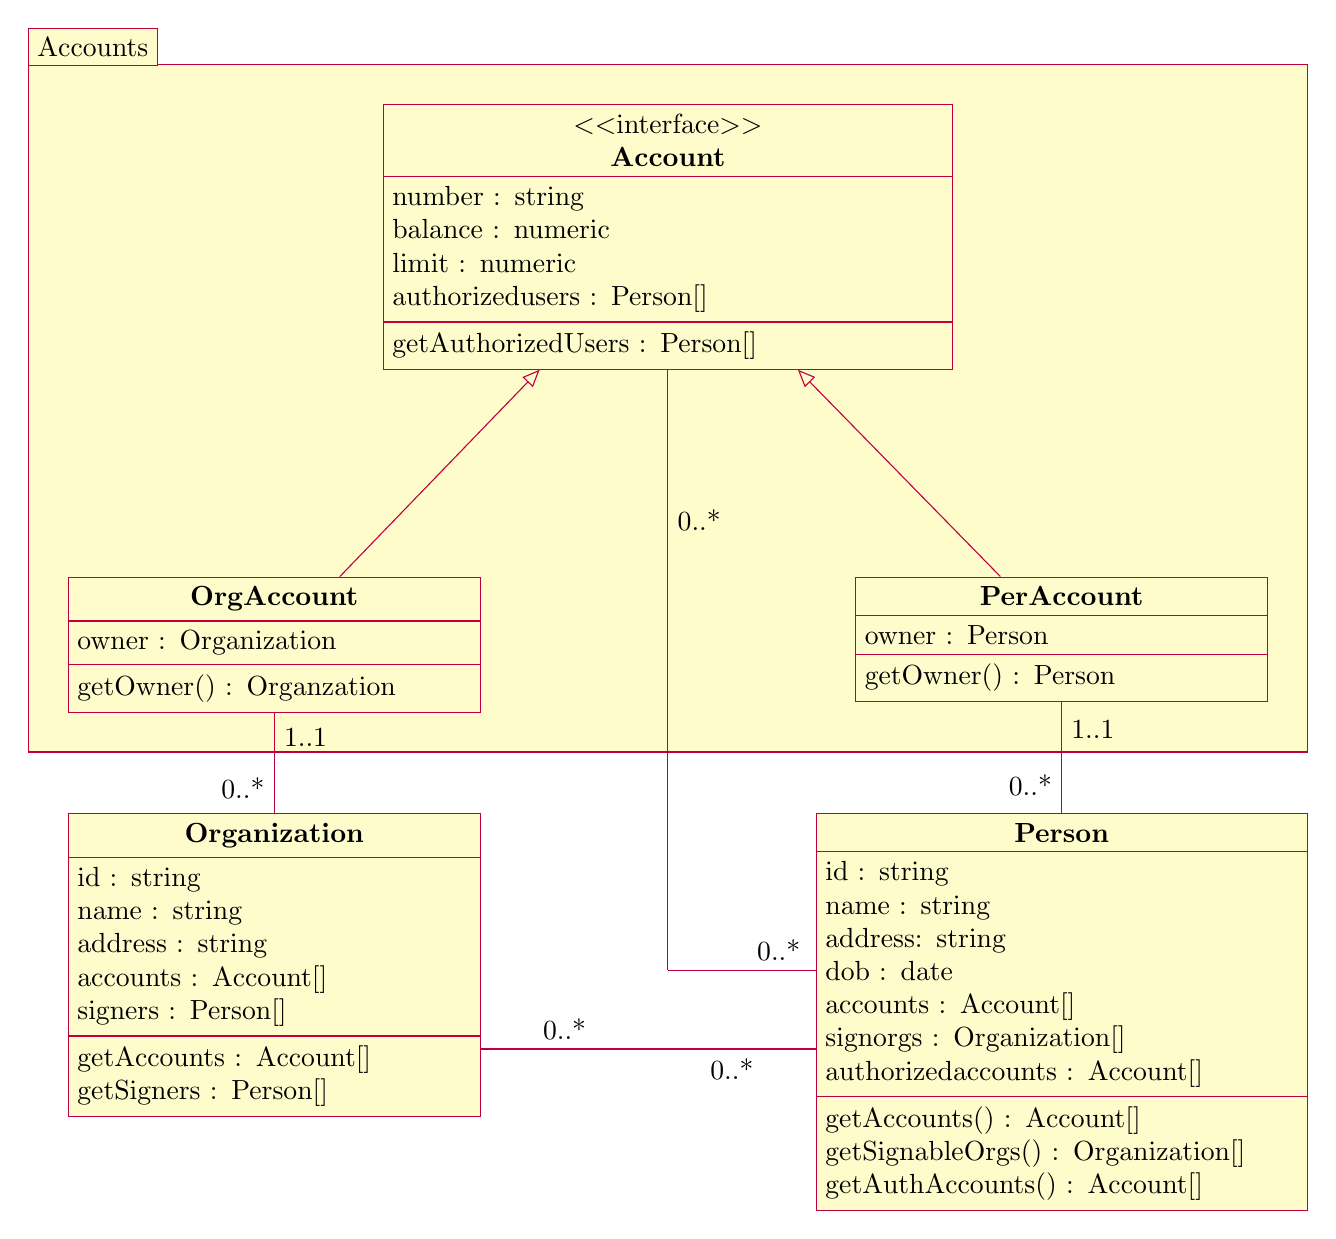
\begin{tikzpicture}
    \begin{package}{Accounts}
        \begin{interface}[text width=7cm]{Account}{0,0}
            \attribute{number : string}
            \attribute{balance : numeric}
            \attribute{limit : numeric}
            \attribute{authorizedusers : Person[]}
            \operation{getAuthorizedUsers : Person[]}
        \end{interface}

        \begin{class}[text width=5cm]{OrgAccount}{-5,-6}
            \attribute{owner : Organization}
            \inherit{Account}
            \operation{getOwner() : Organzation}
        \end{class}

        \begin{class}[text width=5cm]{PerAccount}{5,-6}
            \attribute{owner : Person}
            \inherit{Account}
            \operation{getOwner() : Person}
        \end{class}
    \end{package}
    \begin{class}[text width=5cm]{Organization}{-5,-9}
        \attribute{id : string}
        \attribute{name : string}
        \attribute{address : string}
        \attribute{accounts : Account[]}
        \attribute{signers : Person[]}
        \operation{getAccounts : Account[]}
        \operation{getSigners : Person[]}
    \end{class}
    \begin{class}[text width=6cm]{Person}{5,-9}
        \attribute{id : string}
        \attribute{name : string}
        \attribute{address: string}
        \attribute{dob : date}
        \attribute{accounts : Account[]}
        \attribute{signorgs : Organization[]}
        \attribute{authorizedaccounts : Account[]}
        \operation{getAccounts() : Account[]}
        \operation{getSignableOrgs() : Organization[]}
        \operation{getAuthAccounts() : Account[]}
    \end{class}

    %\association{OrgAccount}{}{1..1}{Organization}{0..*}{}
    \draw [umlcd style] (OrgAccount) -- (Organization) node[near start, right]{1..1} node[near end, left]{0..*};
    %\association{PerAccount}{}{1..1}{Person}{0..*}{}
    \draw [umlcd style] (PerAccount) -- (Person) node[near start, right]{1..1} node[near end, left]{0..*};

    %\association{Organization}{0..*}{}{Person}{}{0..*}

    \draw [umlcd style] (Person.west |- 5, -12) -- (Organization.east |- -5, -12) node[near start, below]{0..*} node[near end, above]{0..*};

    \draw [umlcd style] (Account) -- (0,-11) node[near start, right]{0..*};
    \draw [umlcd style] (Person.west |- 5, -11) -- (0,-11) node[near start, above]{0..*};

\end{tikzpicture}
\caption{UML diagram for CCDB}
\end{figure}


\end{document}
